\section{Introduction}
Modeling is a powerful tool in synthetic biology. It can provide us with an important engineering approach to characterize our pathways quantitatively and predict their performance, thus help us test and modify our design.

Through the dynamic model, we hope to gain insights of the characteristics of our whole circuit's dynamics.

\section{Method}
\subsection{analysis of the problem}
\begin{figure}[h]
\centering
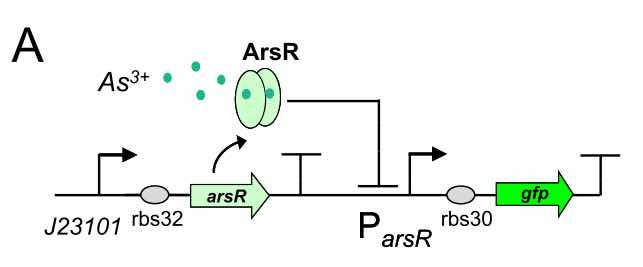
\includegraphics[width=12cm,height=5cm]{1}
\caption{Schematic diagram of plasmid1}
\end{figure}

At the beginning, on the plasmid\#1, the promoter P\textsubscript{arsR} isn't bound with ArsR, thus it is active. ArsR and smURFP are transcribed and translated under the control of the promoters P\textsubscript{arsR\textsubscript{u}} and P\textsubscript{arsR\textsubscript{d}}, with subscript u and d representing upstream and downstream separately. The subscript l of smURFP in the equation means leaky expression without the expression of As\textsuperscript{3+}. As ArsR is expressed gradually, it will bind with the promoter P\textsubscript{arsR} and make it inactive. \cite{pola2018novel}

\begin{equation}
P_{J23104} \stackrel{k_{tx1}}{\longrightarrow} P_{J23104}+mRNA_{ArsR}
\end{equation}
\begin{equation}
mRNA_{ArsR}\stackrel{k_{tl1}}{\longrightarrow} mRNA_{ArsR}+ArsR
\end{equation}
\begin{equation}
P_{arsR} \stackrel{k_{tx2}}{\longrightarrow} P_{arsR} +mRNA_{smURFP}
\end{equation}
\begin{equation}
mRNA_{smURFP} \stackrel{k_{tl2}}{\longrightarrow} mRNA_{smURFP}+ smURFP
\end{equation}

\begin{equation}
ArsR+P_{arsR} \xrightleftharpoons[k_{-b1}]{k_{b1}}ArsR*P_{arsR} 
\end{equation} 
On the plasmid\#2, the fusion protein of dCas9 and RNAP(RNA polymerase) are produced after transcription and translation, and $sgRNA$ is produced after transcription.


\begin{equation}
P_{tet} \stackrel{k_{tx3}}{\longrightarrow} P_{tet} +mRNA_{dCas9-RNAP}
\end{equation}
\begin{equation}
mRNA_{dCas9-RNAP} \stackrel{k_{tl3}}{\longrightarrow} mRNA_{dCas9-RNAP}+dCas9-RNAP
\end{equation}

\begin{equation}
P_{tet} \stackrel{k_{tx4}}{\longrightarrow} P_{tet} +sgRNA
\end{equation}

\begin{figure}[h]
	\centering
	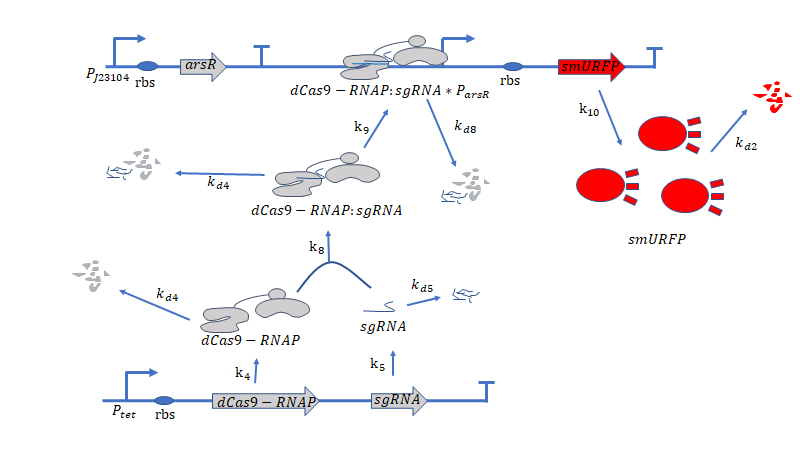
\includegraphics[width=12cm,height=5cm]{2}
	\caption{Schematic diagram of dCas9/RNAP}
\end{figure}

dCas9(*RNAP) can bind with its target DNA sequence without cutting, which is at the upstream of the promoter P\textsubscript{arsR\textsubscript{d}}. Simultaneously, dCas9 can lead RNAP to bind with the promoter P\textsubscript{arsR\textsubscript{d}} and enhance the transcription of smURFP. However, because the promoter P\textsubscript{arsR\textsubscript{d}} has already bound with ArsR, as a result, RNAP can't bind with the promoter P\textsubscript{arsR\textsubscript{d}} \cite{bikard2013programmable}. \\ 

However, at the presence of As\textsuperscript{3+}, it can bind with ArsR, then dissociate ArsR and P\textsubscript{arsR\textsubscript{d}} , which makes the combination of RNAP and P\textsubscript{arsR\textsubscript{d}} possible. \\

(Declaration: [dCas9/RNAP] = [dCas9] = [RNAP]; [P\textsubscript{arsR\textsubscript{d}}] = [P\textsubscript{arsR\textsubscript{u}}] = 0.5{[P\textsubscript{arsR}]})

\begin{equation}
ArsR +As^{3+}\xrightleftharpoons[k_{-b2}]{k_{b2}}As^{3+}*ArsR
\end{equation}

\begin{equation}
ArsR*P_{arsR} +As^{3+}\xrightleftharpoons[k_{-b3}]{k_{b3}}P_{arsR}+ As^{3+}*ArsR
\end{equation}

\begin{equation}
dCas9-RNAP+sgRNA\xrightleftharpoons[k_{-b4}]{k_{b4}} dCas9-RNAP:sgRNA
\end{equation}

\begin{equation}
dCas9-RNAP:sgRNA+P_{arsR}\xrightleftharpoons[k_{-b5}]{k_{b5}} dCas9-RNAP:sgRNA*P_{arsR}
\end{equation}

\begin{equation}
dCas9-RNAP:sgRNA*P_{arsR}\stackrel{k_{b6}}{\longrightarrow} dCas9-RNAP:sgRNA*P_{arsR}+smURFP
\end{equation}
\\
We then take degradation into account:\\
\begin{equation}
\text{ArsR}\stackrel{k_{d1}}{\longrightarrow}Ø
\end{equation}
\begin{equation}
\text{smURFP}\stackrel{k_{d2}}{\longrightarrow}Ø
\end{equation}
\begin{equation}
\text{ArsR*P\textsubscript{arsR}}\stackrel{k_{d3}}{\longrightarrow} P\textsubscript{arsR}
\end{equation}
\begin{equation}
\text{As\textsuperscript{3+}*ArsR} \stackrel{k_{d4}}{\longrightarrow}\text{As\textsuperscript{3+}}
\end{equation}
\begin{equation}
\text{dCas9*RNAP}\stackrel{k_{d5}}{\longrightarrow}Ø
\end{equation}
\begin{equation}
\text{sgRNA}\stackrel{k_{d6}}{\longrightarrow}Ø
\end{equation}
%\begin{equation}
%dCas9-RNAP:sgRNA\stackrel{k_{d7}}{\longrightarrow}dCas9-RNAP
%\end{equation}
\begin{equation}
\text{dCas9*RNAP:sgRNA}\stackrel{k_{d7}}{\longrightarrow}Ø
\end{equation}
%\begin{equation}
%dCas9-RNAP:sgRNA*P_{arsR}\stackrel{k_{d8}}{\longrightarrow}dCas9-RNAP+P_{arsR}
%\end{equation}
\begin{equation}
\text{dCas9*RNAP:sgRNA*P\textsubscript{arsR}}\stackrel{k_{d8}}{\longrightarrow}P\textsubscript{arsR}
\end{equation}
\begin{equation}
mRNA_{ArsR}\stackrel{k_{d9}}{\longrightarrow}Ø
\end{equation}
\begin{equation}
mRNA_{smURFP}\stackrel{k_{d10}}{\longrightarrow}Ø
\end{equation}
\begin{equation}
mRNA_{dCas9-RNAP}\stackrel{k_{d11}}{\longrightarrow}Ø
\end{equation}
\\
\subsection{Differential Equations}
Applying mass action kinetic laws, we obtain the following set of differential equations. The several complexes involved:ArsR*P\textsubscript{arsR} , As\textsuperscript{3+}*ArsR, dCas9*RNAP, dCas9*RNAP:sgRNA, dCas9*RNAP:sgRNA*P\textsubscript{arsR}, are respectively abbreviated as $cplx_1$, $cplx_2$, $cplx_3$, $cplx_4$, $cplx_5$.
\begin{equation}
\frac{d[ArsR]}{dt}=k_{tl1}[mRNA_{ArsR}]-k_{d1}[ArsR]\tag{1}
\end{equation}
\begin{equation}
\frac{d[smURFP]}{dt}=k_{tl2}[mRNA_{smURFP}]+k_{b6}[cplx_5]-k_{d2}[smuRFP]\tag{2}
\end{equation}
\begin{equation}
\frac{d[cplx_1]}{dt}=k_{b1}[ArsR][P_{arsR}]-k_{b3}[As^{3+}][[cplx_1]-k_{d3}[cplx_1] \tag{3}
\end{equation}
\begin{equation}
\frac{d[cplx_3]}{dt}=k_{tl3}[mRNA_{dcplx1}]-k_{b4}[cplx_3][sgRNA]-k_{d5}[cplx_3] \tag{4}
\end{equation}
\begin{equation}
\frac{d[sgRNA]}{dt}=k_{tx4}[P_{tet}]-k_{b4}[cplx_3][sgRNA]-k_{d6}[sgRNA] \tag{5}
\end{equation}
\begin{equation}
\frac{d[cplx_2]}{dt}=k_{b2}[As^{3+}][ArsR]+k_{b3}[As^{3+}][cplx_1]-k_{d4}[cplx_2] \tag{6}
\end{equation}
\begin{equation}
\frac{d[As^{3+}]}{dt}=-k_{2}[As^{3+}][ArsR]-k_{b3}[As^{3+}][cplx_1] \tag{7}
\end{equation}
\begin{equation}
\frac{d[cplx_4]}{dt}=k_{b4}[cplx_3][sgRNA]-k_{b5}[cplx_4][P_{arsR}]-k_{d7}[cplx_4]\tag{8}
\end{equation}
\begin{equation}
\frac{d[cplx_5]}{dt}=k_{b5}[cplx_4][P_{arsR}]-k_{d8}[cplx_5]\tag{9}
\end{equation} 
\begin{equation}
\frac{d[P_{J23104}]}{dt}=0\tag{10}
\end{equation} 
\begin{equation}
\frac{d[P_{ArsR}]}{dt}=0\tag{11}
\end{equation} 
\begin{equation}
\frac{d[P_{tet}]}{dt}=0\tag{12}
\end{equation} 
\begin{equation}
\frac{d[mRNA_{ArsR}]}{dt}=k_{tx1}[P_{J12304}]-k_{d9}[[mRNA_{ArsR}] \tag{13}
\end{equation}
\begin{equation}
\frac{d[mRNA_{smURFP}]}{dt}=k_{tx2}[P_{arsR}]-k_{d10}[[mRNA_{smURFP}] \tag{14}
\end{equation}
\begin{equation}
\frac{d[mRNA_{dcplx1}]}{dt}=k_{tx3}[P_{tet}]-k_{d11}[mRNA_{dcplx1}] \tag{15}
\end{equation}
\\\\
\begin{table}[htbp]
	\centering
	\caption{\label {tab:test} Parameters}
	\begin{tabular}{ccccccccccccccccccccc}
		\toprule
		Rate constants & Value& units & source \\
		\midrule
		$k_{tx1}$ & 1.5e-2&$s^{-1} $& Berset et al. \\
		$k_{tl1}$ & 7.33e-2 &$s^{-1} $& Berset et al.\\
		$k_{tx2}$ & 1.5e-2 & $s^{-1}$ & Berset et al.\\
		$k_{tl2} $&1.84e-13&$s^{-1}$& Berset et al.\\
		$k_{b1} $& 1e4   & $nM^{-1}s^{-1}$ &2006 iGEM Edinburgh  \\
		$k_{-b1}$ & 0.65    & $nM^{-1}s^{-1}$ &2006 iGEM Edinburgh   \\
		$k_{tx3}$& 5e-4 &$s^{-1}$&Estimated to be slow in comparison to $k_{tx4} $\\
		$k_{tl3} $& 0.072   & $s^{-1}$ & calculated from Eyal Karzbrun et al.  \\
		$k_{tx4} $& 1.33e-3 &$s^{-1}$&2007 iGEM Imperial College London \\
		$k_{b2} $& 1e3   & $nM^{-1}s^{-1}$ &2006 iGEM Edinburgh  \\
		$k_{-b2} $& 0.65    & $nM^{-1}s^{-1}$ &2006 iGEM Edinburgh   \\
		$k_{b3}  $&1.26e4 &$nM^{-1}s^{-1}$ & berset et al. \\
		$k_{b4}$&1.6e-2& $nM^{-1}s^{-1}$& 2017iGEM Munich\\
		$k_{b5} $&1.66e-5&$nM^{-1}s^{-1}$&  2017GEM Munich\\ 
		$k_{b6}$&4e-5&$s^{-1} $& Estimated to be slow in comparison to k2 \\
		$k_{d1} $& 3.07e-3&$s^{-1} $ & Berset et al.\\
		$k_{d2}$&1e-5&$s^{-1} $ & Berset et al.\\
		$k_{d3}$&1e-3&$s^{-1} $ & Berset et al.\\
		$k_{d4}$&1.53e-3&$s^{-1} $  & Berset et al.\\
		$k_{d5} $& 2e-2&$s^{-1} $& Estimated to be fast in comparison to kd1\\
		$k_{d6}$&7.62e-3&$s^{-1} $&  Estimated according to 	
		Berset et al.\\
		$k_{d7}$& 1e-2&$s^{-1} $&  Estimated to be slow in comparison to kd5\\
		$k_{d8}$&1e-1&$s^{-1} $&  Estimated to be slow in comparison to kd7\\
		$k_{d9}$&2.81e-3  & $ns^{-1}$ & Berset et al.  \\
		$k_{d10} $ &7.62e-3 &$s^{-1}$ & Berset et al. \\
		$k_{d11}$& 8e-4& $s^{-1}$& Estimated to be slow in comparison to $k_{d9}$ \\
		\bottomrule
	\end{tabular}
\end{table}



\subsection{simulation }
\begin{figure}[h]
	\centering
	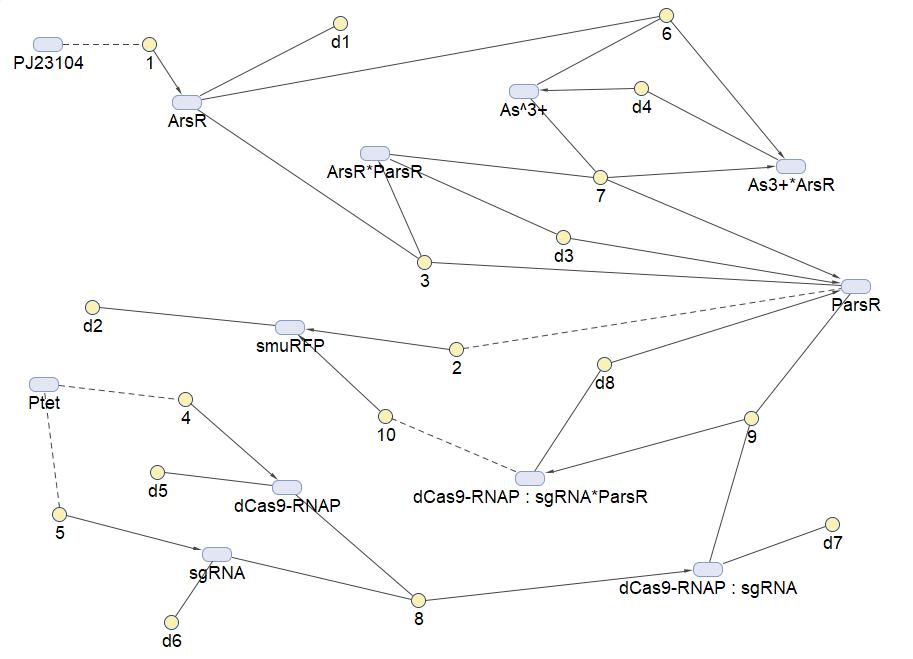
\includegraphics[width=10cm,height=7cm]{screenshot003}	
	\caption{reaction map generated from the reaction set above using SimBiology Toolbox}
\end{figure}
SimBiology toolbox provides functions for modeling, simulating, and analyzing biochemical pathways on basis of the powerful computing engine of Matlab.

\begin{figure}[h]
	\centering
	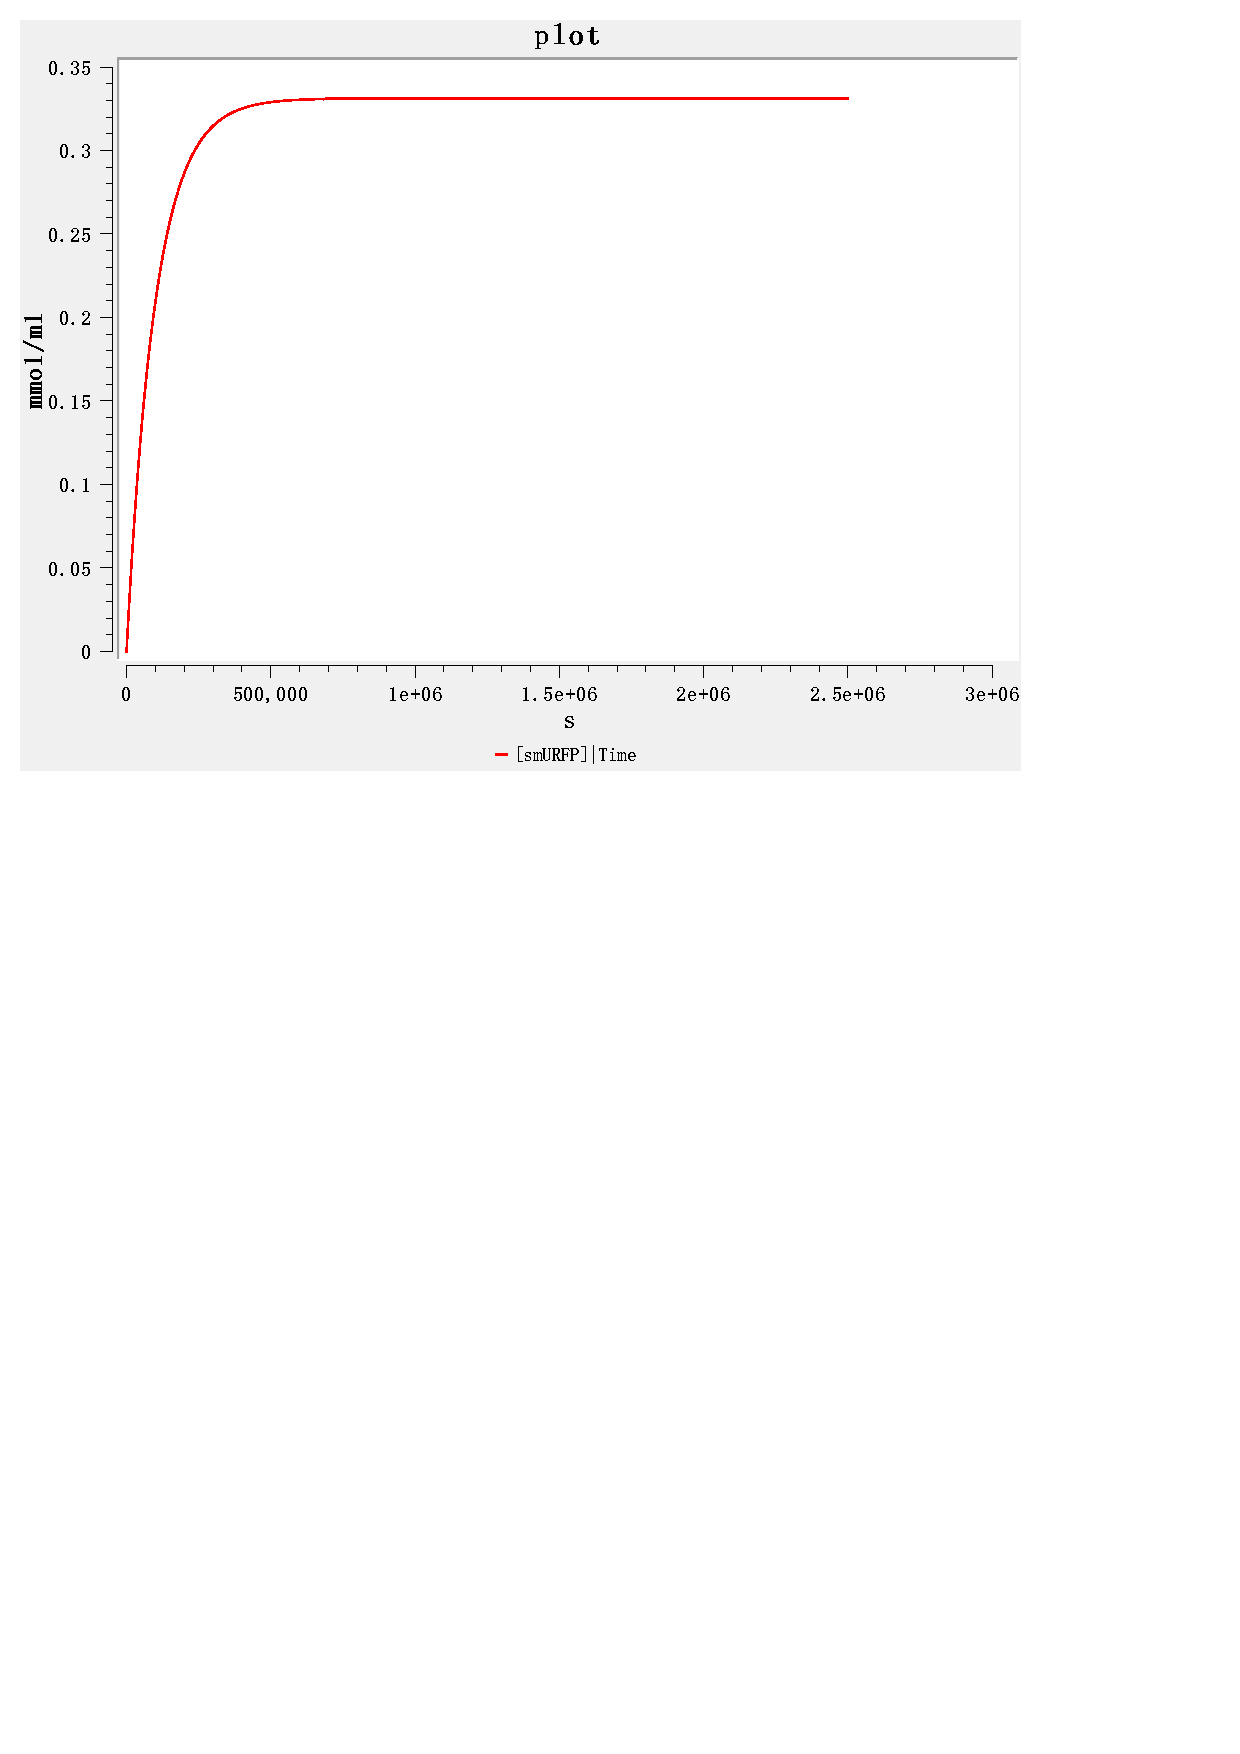
\includegraphics[width=10cm,height=10cm]{smuRFP}
	\caption{Schematic diagram of smURFP fluorescence by COPASI}
\end{figure}



COPASI is freeware developed withcollaboration of VBI and EMLR. It provides
almost the same functions as SimBiology, though not quite powerful. But compared with SimBiology, it provides a friendly user interface for model analysis, such as parameter estimation,and parameter scan.

Through the figure, we can see that the smURFP fluorescence gradually increased and then reached a steady state after a period of time  in the presence of arsenic ions.

\subsection{sensitivity }
\subsection{sensitivity }
A good biosystem should be with a stability towards fluctuations in parameters. And  a  good model should also reflect this and hence a test for robustness can be an important test of the model.
Robustness analysis can also pinpoint which reactions/parameters that are important for obtaining a specific biological behavior. A simple measure for sensitivity is to measure the relative change of a system feature due to a change in a parameter. As for our model, the feature can be the equilibrium concentration of the smuRFP,C for which the sensitivity (S) to a parameter k is:
\begin{equation}
S=\frac{\frac{dC}{C}}{\frac{dk}{k}}=\frac{dC}{dk}\frac{k}{c}\approx \frac{\Delta C}{\Delta k}\frac{k}{c}
\end{equation}
The Matlab scripts used for sensitivity analysis see attached.
\begin{figure}
	\centering
	\begin{varwidth}[t]{\textwidth}
		\vspace{0pt}
		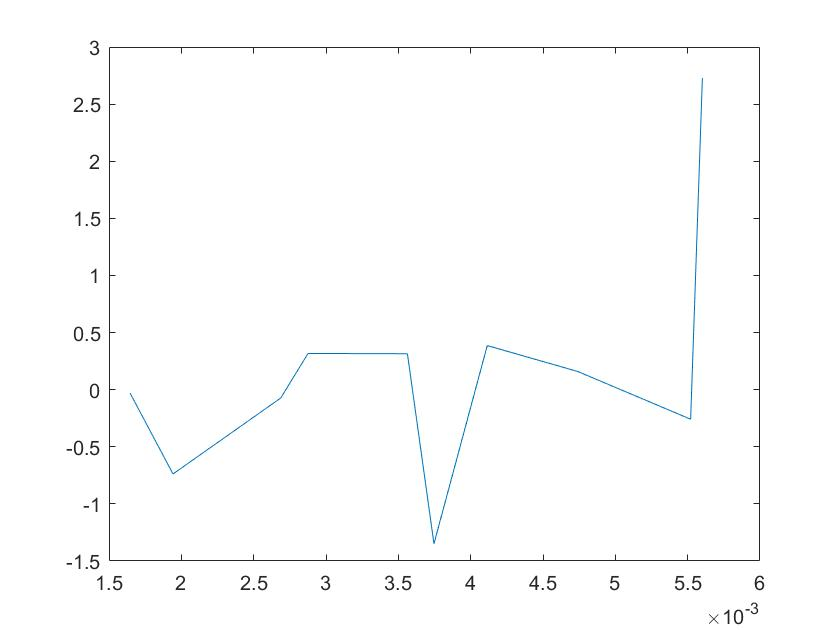
\includegraphics[height=4cm]{s1.jpg}
	\end{varwidth}%
	\caption{sensitivity of k1}
	%\qquad 
	\begin{varwidth}[t]{\textwidth}
		\vspace{0pt}
		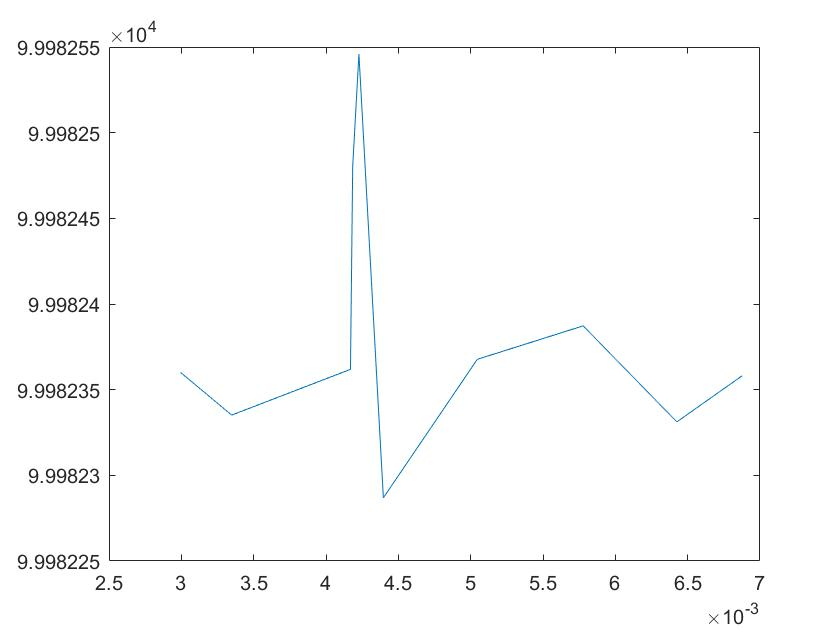
\includegraphics[height=4cm]{s2.jpg}
	\end{varwidth}
	\caption{sensitivity of k2}
	\begin{varwidth}[t]{\textwidth}
		\vspace{0pt}
		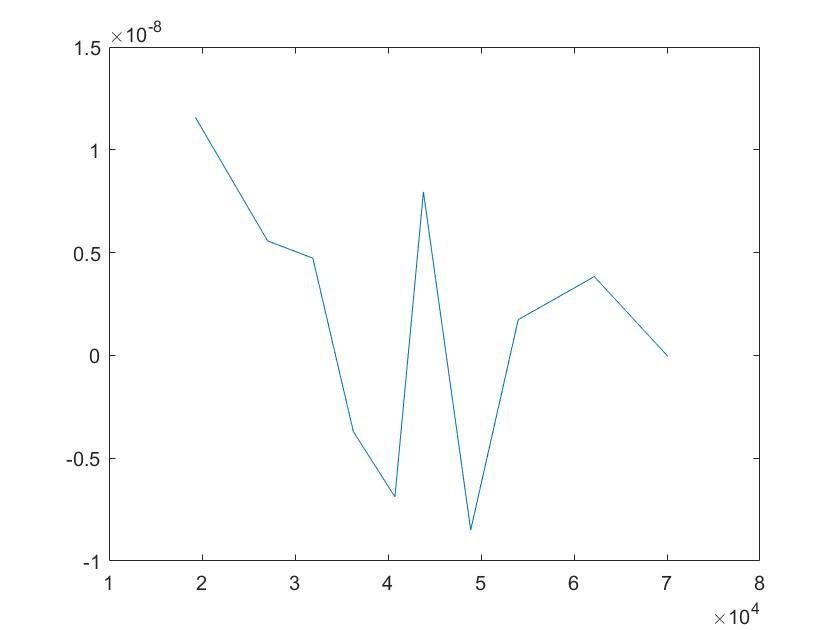
\includegraphics[height=4cm]{s3.jpg}
	\end{varwidth}
	\caption{sensitivity of k3}
	\begin{varwidth}[t]{\textwidth}
		\vspace{0pt}
		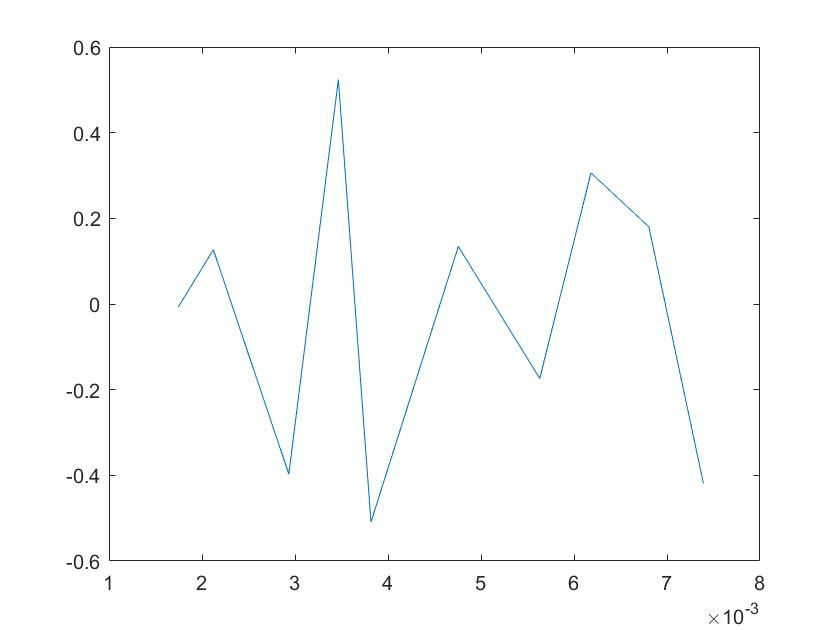
\includegraphics[height=4cm]{s4.jpg}
	\end{varwidth}
	\caption{sensitivity of k4}
	\begin{varwidth}[t]{\textwidth}
		\vspace{0pt}
		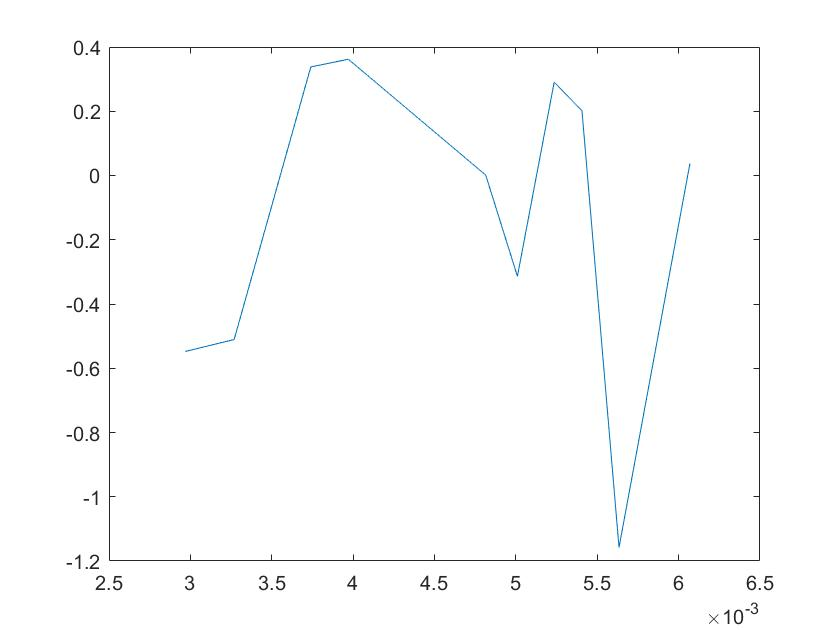
\includegraphics[height=4cm]{s5.jpg}
	\end{varwidth}
	\caption{sensitivity of k5}
	\begin{varwidth}[t]{\textwidth}
		\vspace{0pt}
		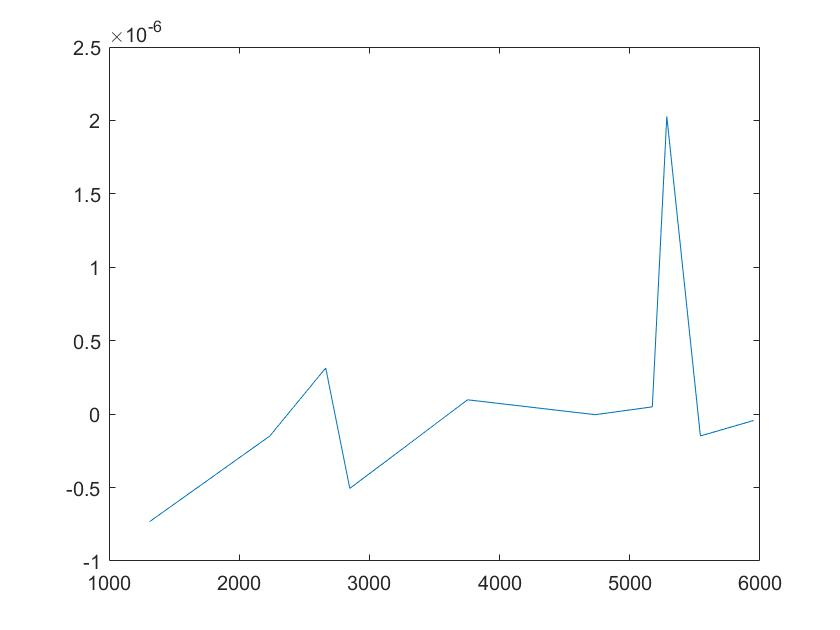
\includegraphics[height=4cm]{s6.jpg}
	\end{varwidth}
	\caption{sensitivity of k6}
	\begin{varwidth}[t]{\textwidth}
		\vspace{0pt}
		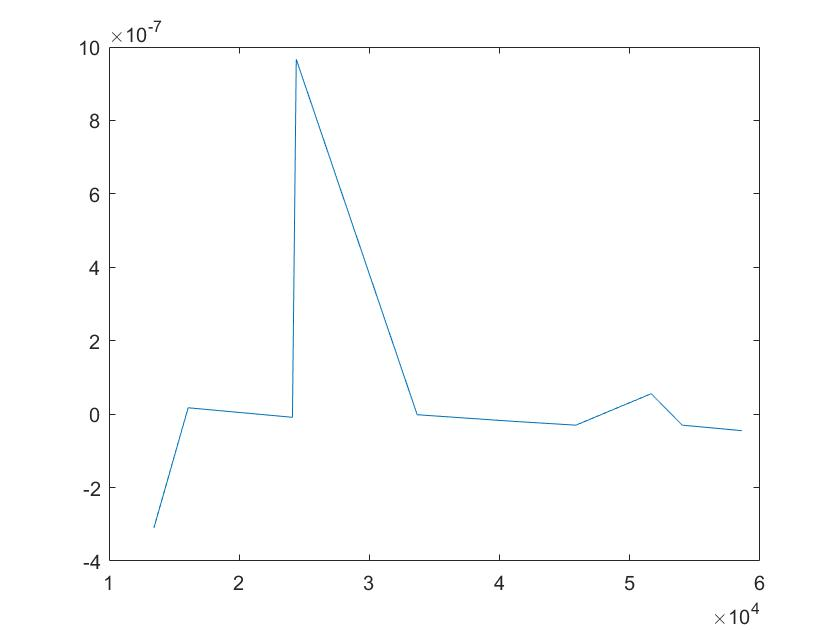
\includegraphics[height=4cm]{s7.jpg}
	\end{varwidth}
	\caption{sensitivity of k7}
	\begin{varwidth}[t]{\textwidth}
		\vspace{0pt}
		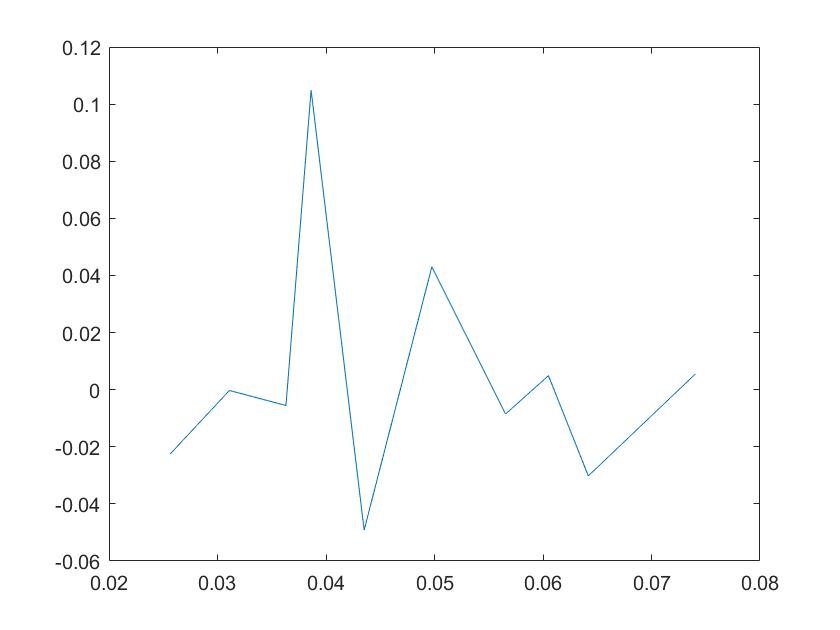
\includegraphics[height=4cm]{s8.jpg}
	\end{varwidth}
	\caption{sensitivity of k8}
	\begin{varwidth}[t]{\textwidth}
		\vspace{0pt}
		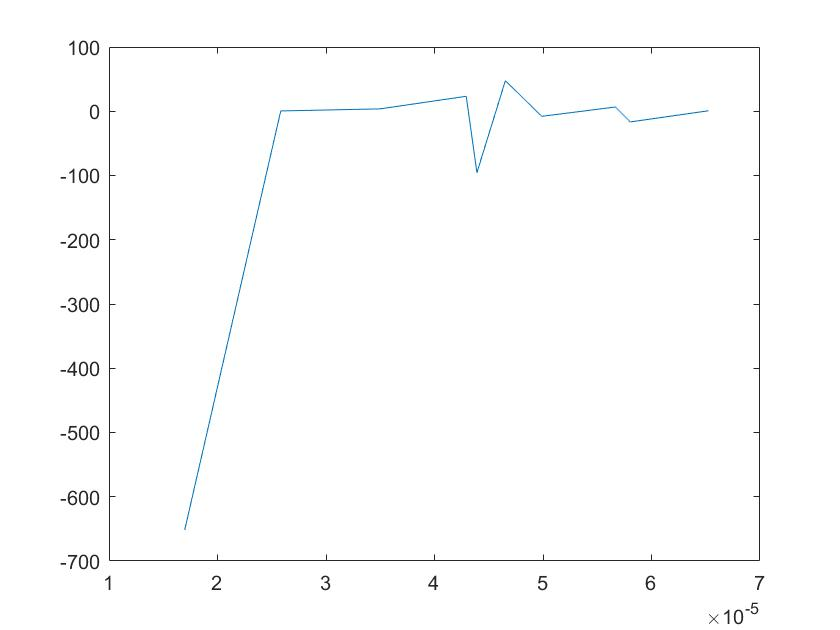
\includegraphics[height=4cm]{s9.jpg}
	\end{varwidth}
	\caption{sensitivity of k9}
	\begin{varwidth}[t]{\textwidth}
		\vspace{0pt}
		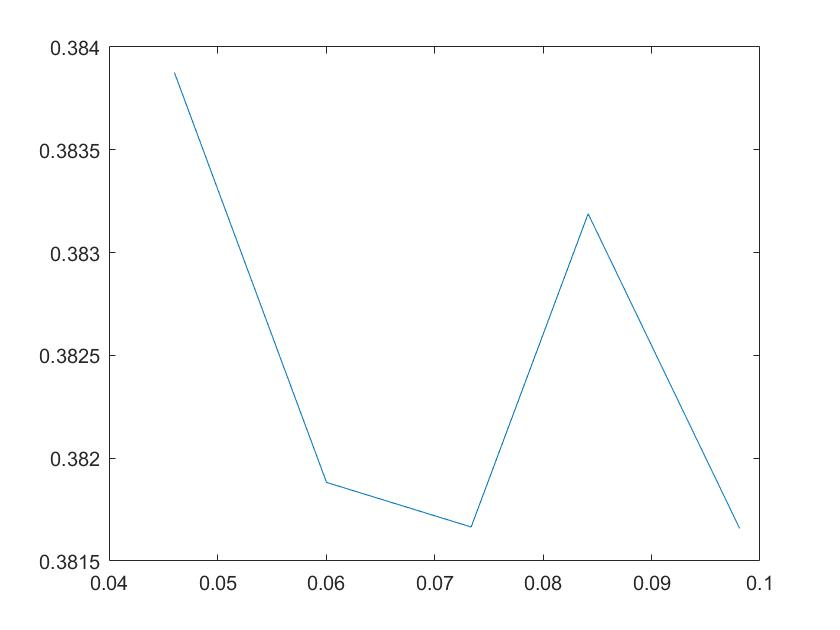
\includegraphics[height=4cm]{s10.jpg}
	\end{varwidth}
	\caption{sensitivity of k10}
	\begin{varwidth}[t]{\textwidth}
		\vspace{0pt}
		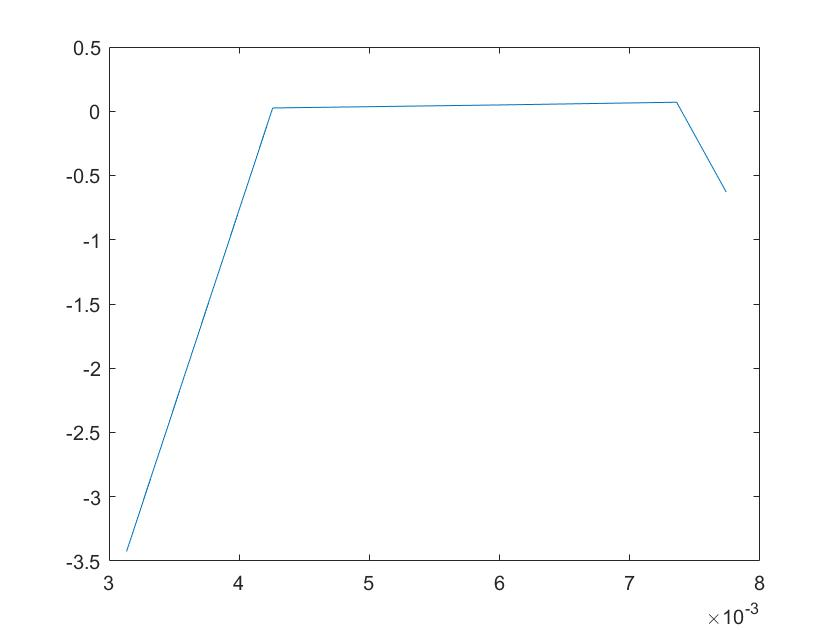
\includegraphics[height=4cm]{sd1.jpg}
	\end{varwidth}
	\caption{sensitivity of kd1}
	\begin{varwidth}[t]{\textwidth}
		\vspace{0pt}
		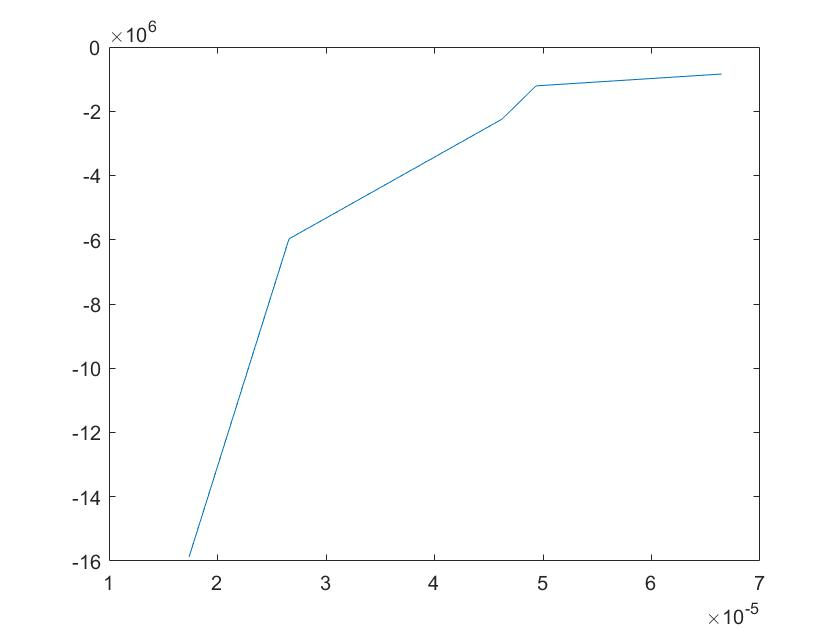
\includegraphics[height=4cm]{sd2.jpg}
	\end{varwidth}
	\caption{sensitivity of kd2}
	\begin{varwidth}[t]{\textwidth}
		\vspace{0pt}
		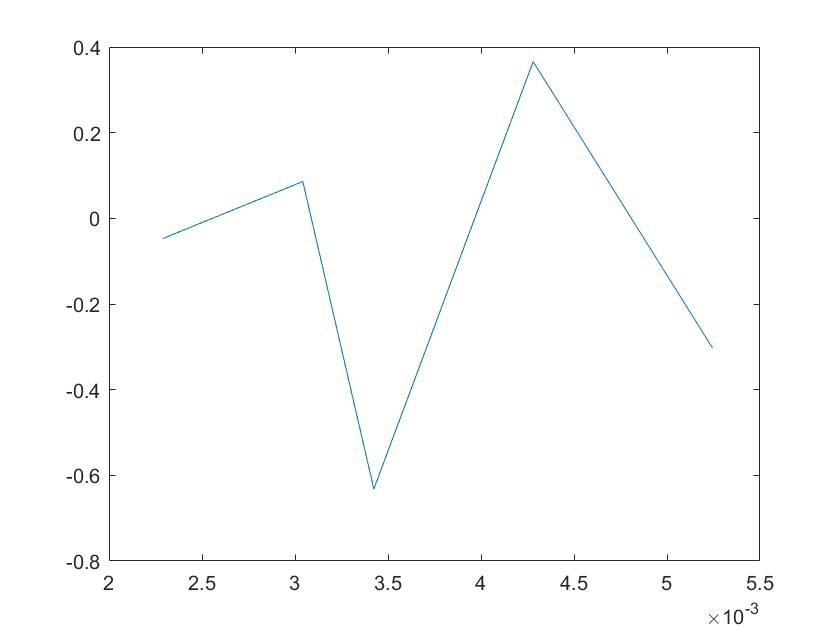
\includegraphics[height=4cm]{sd3.jpg}
	\end{varwidth}
	\caption{sensitivity of kd3}
	\begin{varwidth}[t]{\textwidth}
		\vspace{0pt}
		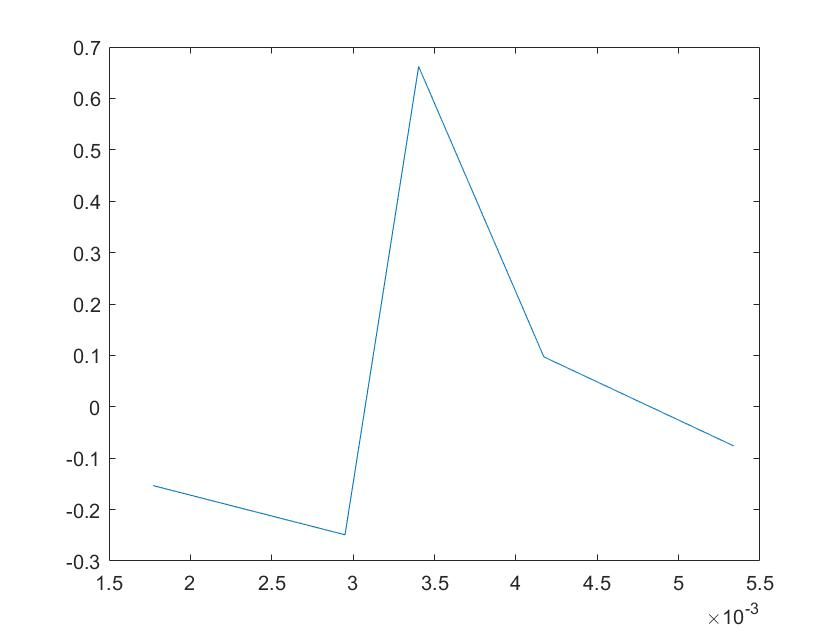
\includegraphics[height=4cm]{sd4.jpg}
	\end{varwidth}
	\caption{sensitivity of kd4}
	\begin{varwidth}[t]{\textwidth}
		\vspace{0pt}
		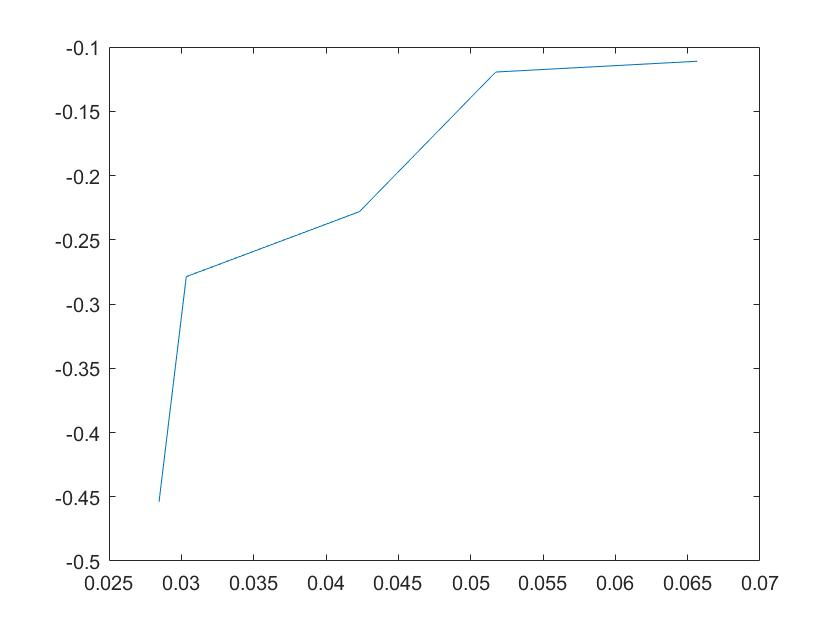
\includegraphics[height=4cm]{sd5.jpg}
	\end{varwidth}
	\caption{sensitivity of kd5}
	\begin{varwidth}[t]{\textwidth}
		\vspace{0pt}
		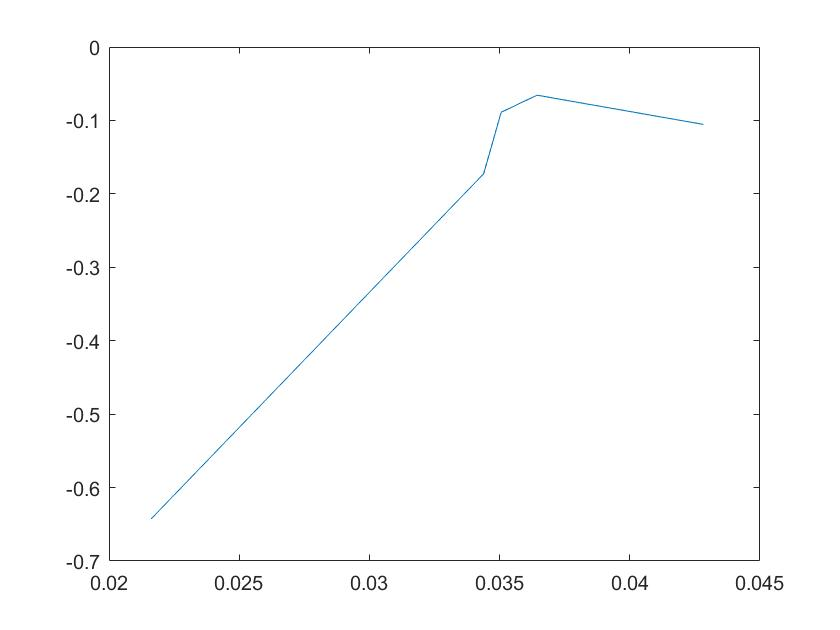
\includegraphics[height=4cm]{sd6.jpg}
	\end{varwidth}
	\caption{sensitivity of kd6}
	\begin{varwidth}[t]{\textwidth}
		\vspace{0pt}
		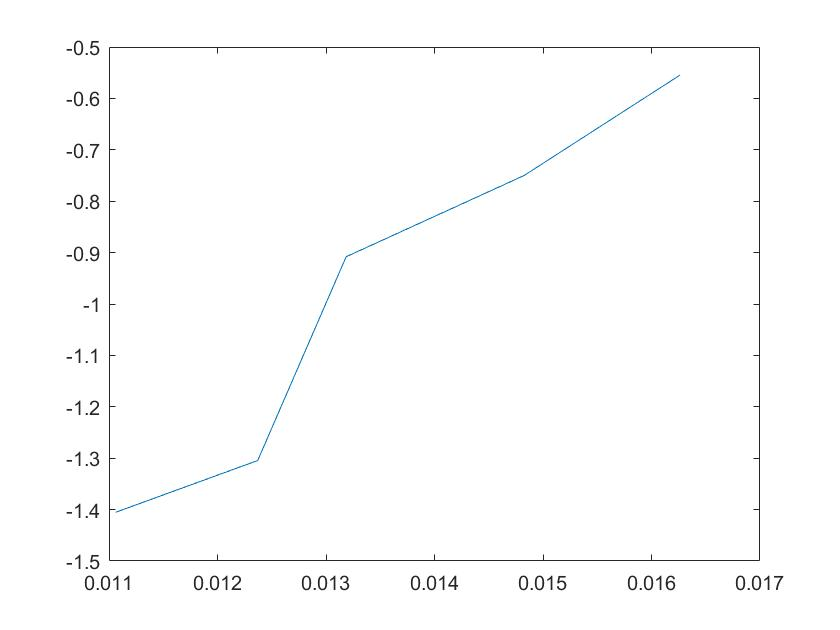
\includegraphics[height=4cm]{sd7.jpg}
	\end{varwidth}
	\caption{sensitivity of kd7}
	\begin{varwidth}[t]{\textwidth}
		\vspace{0pt}
		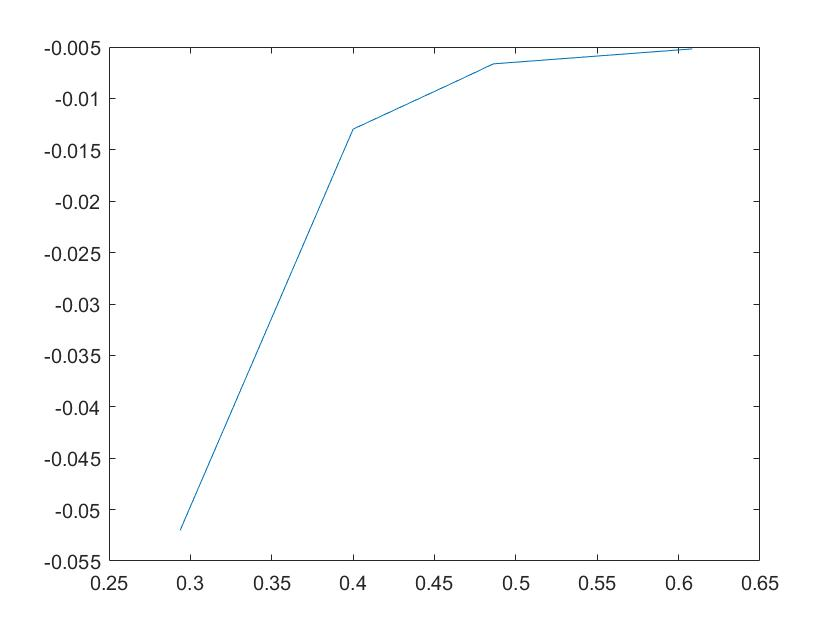
\includegraphics[height=4cm]{sd8.jpg}
	\end{varwidth}
	\caption{sensitivity of kd8}
\end{figure}

\subsection{modification of the model}
The results are  not very satisfactory, and we suspect that it may be due to the simplification of the two processes of transcription and translation when producing proteins into a one-step process.So we take the mRNA into account, and then the reaction (1) to (4) four reactions should be replaced by the  following 6 reaction equations:
\begin{equation}
P_{J23104} \stackrel{k_{1'}}{\longrightarrow} P_{J23104}+mRNA_{ArsR}
\end{equation}
\begin{equation}
mRNA_{ArsR}\stackrel{k_{2'}}{\longrightarrow} mRNA_{ArsR}+ArsR
\end{equation}
\begin{equation}
P_{arsR} \stackrel{k_{3'}}{\longrightarrow} P_{arsR} +mRNA_{smURFP}
\end{equation}
\begin{equation}
mRNA_{smURFP} \stackrel{k_{4'}}{\longrightarrow} mRNA_{smURFP}+ smURFP
\end{equation}
\begin{equation}
P_{tet} \stackrel{k_{5'}}{\longrightarrow} P_{tet} +mRNA_{dCas9-RNAP}
\end{equation}
\begin{equation}
mRNA_{dCas9-RNAP} \stackrel{k_{6'}}{\longrightarrow} mRNA_{dCas9-RNAP}+dCas9-RNAP
\end{equation}
And the reaction equation set for the degradation of the reaction substance should also be added to the following two reaction equations.
\begin{equation}
mRNA_{ArsR}\stackrel{k_{d9}}{\longrightarrow}Ø
\end{equation}
\begin{equation}
mRNA_{smURFP}\stackrel{k_{d10}}{\longrightarrow}Ø
\end{equation}
\begin{equation}
mRNA_{dCas9-RNAP}\stackrel{k_{d11}}{\longrightarrow}Ø
\end{equation}
Added parameter values:
\begin{table}[htbp]
	\centering
	\caption{\label {tab:test} Parameters}
	\begin{tabular}{cccccccccccccccccc}
		\toprule
		Rate constants & Value& units & source \\
		\midrule
		k1' & 1.5e-2&$s^{-1} $& Berset et al. \\
		k2' & 7.33e-2 &$s^{-1} $& Berset et al.\\
		k3' & 1.5e-2 & $s^{-1}$ & Berset et al.\\
		k4' &1.84e-13&$s^{-1}$& Berset et al.\\
		k5'&  1.33e-3  & $s^{-1}$ & 	iGEM 2007 Imperial College London \\
		k6' &   & $min^{-1}$ &   \\
		kd9&2.81e-3  & $s^{-1}$ & Berset et al.  \\
		kd10  &7.62e-3 &$s^{-1}$ & Berset et al. \\
		kd11& & $s^{-1}$& \\
		
		\bottomrule
	\end{tabular}
\end{table}

\subsection{a bold assumption}
Since the goal of our project is to try to increase the sensitivity of biosensors by introducing a complex of dcas9-RNAP and sgRNA, and the purpose of our model is to explore whether this complex is effective. So why not assume a reasonable and large enough concentration value for this complex. We use the concentration of glyceraldehyde-3-phosphate dehydrogenase A as the assumed concentration. Glyceraldehyde 3 phosphate dehydrogenase A (gapA) is a key enzyme in the glycolytic pathway, and the gene encoding this enzyme is a housekeeping gene in E. coli cells with high expression levels. We found in the literature that the protein mass of gapA is 48645fg/cell, and its molecular weight is 35492 Da.The amount of abundance of Glyceraldehyde 3 phosphate dehydrogenase A protein per cell can be calculated as follows:

\begin{displaymath}
n=\frac{m}{M}=\frac{48645*10^{-15}g}{35492g/mol}=1.37*10^{-15}mol
\end{displaymath}
As for the size of E. coli, we found relevant data from the literature, see the figure below.

\begin{figure}[!htbp]
	\centering
	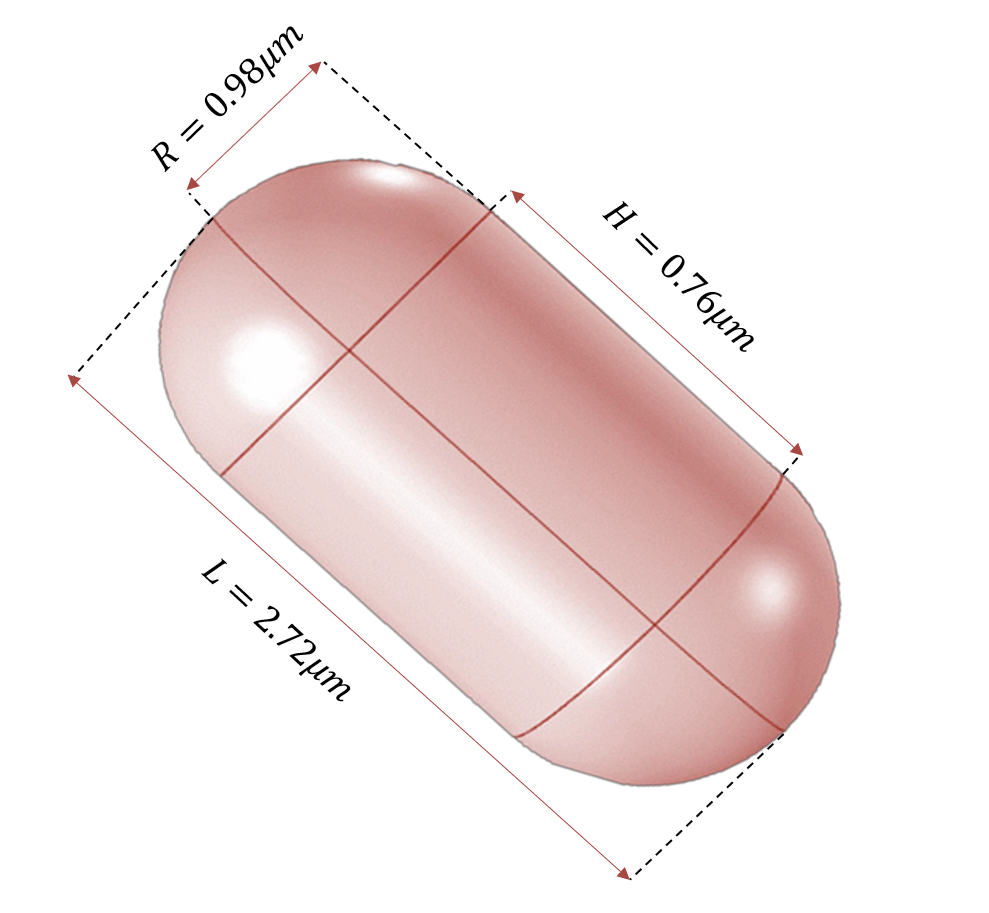
\includegraphics[width=7cm,height=7cm]{dc}
	\caption{size of E. coli}
\end{figure}

The volume of E. coli can be calculated as follows:
\begin{displaymath}
V_{E.coli}=\frac{4}{3} \pi R^3+\pi R^2H=\frac{4}{3} \pi (0.98\mu m)^3+\pi (0.98\mu m)^2(0.76\mu m)=6.24\mu m^3=6.24*10^{-15}L
\end{displaymath}

Then the concentration of Glyceraldehyde 3 phosphate dehydrogenase A protein in the cell can be determined:
\begin{displaymath}
c=\frac{n}{V_{E.coli}}=\frac{1.37*10^{-15}mol}{6.24*10^{-15}L}=0.22mol/L
\end{displaymath}
With this concentration, we got very nice results:

\begin{figure}[!htbp]
	\centering
	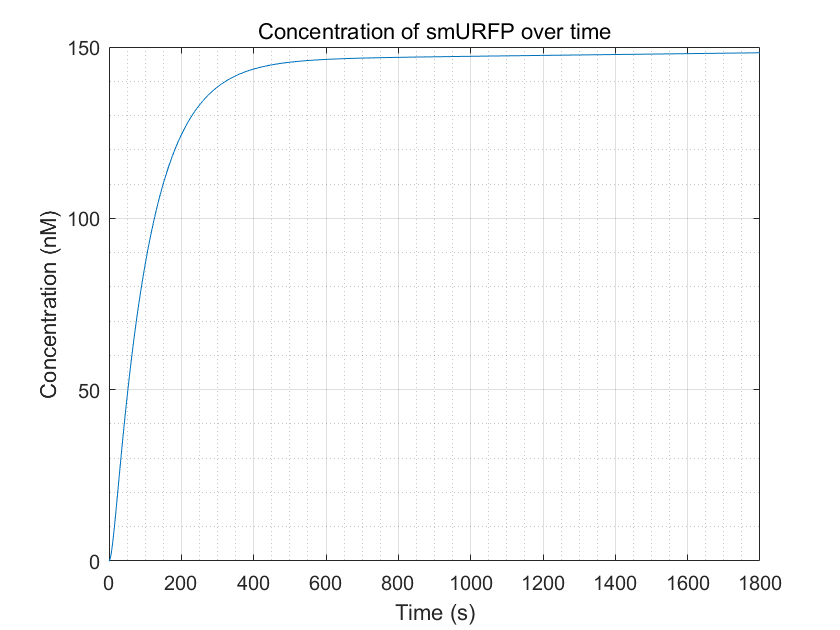
\includegraphics[width=7cm,height=7cm]{23}
	\caption{Schematic diagram of smURFP fluorescence}
\end{figure}
Compared to the diagram without introducing dcas9:
\begin{figure}[!htbp]
	\centering
	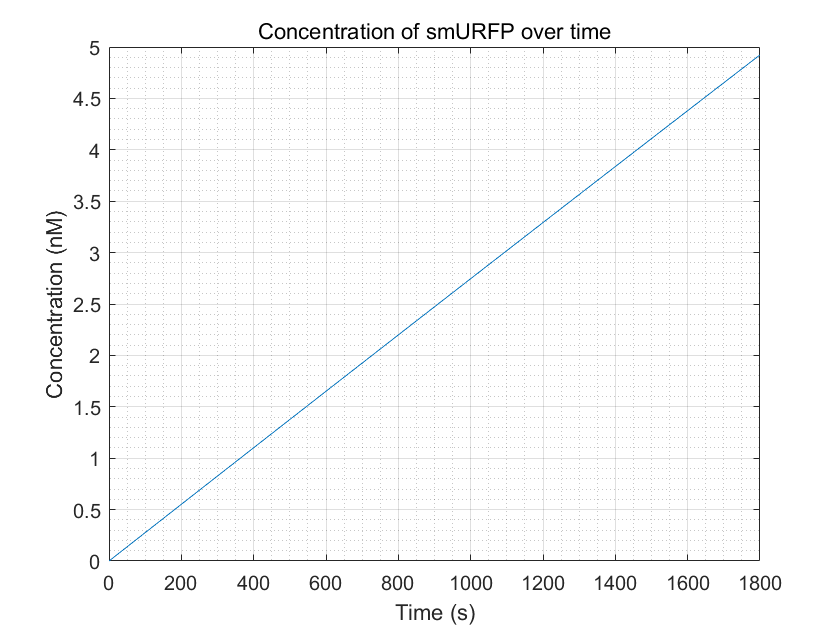
\includegraphics[width=7cm,height=7cm]{21}
	\caption{smURFP fluorescence within a reasonable time frame}
\end{figure}
\begin{figure}[!htbp]
	\centering
	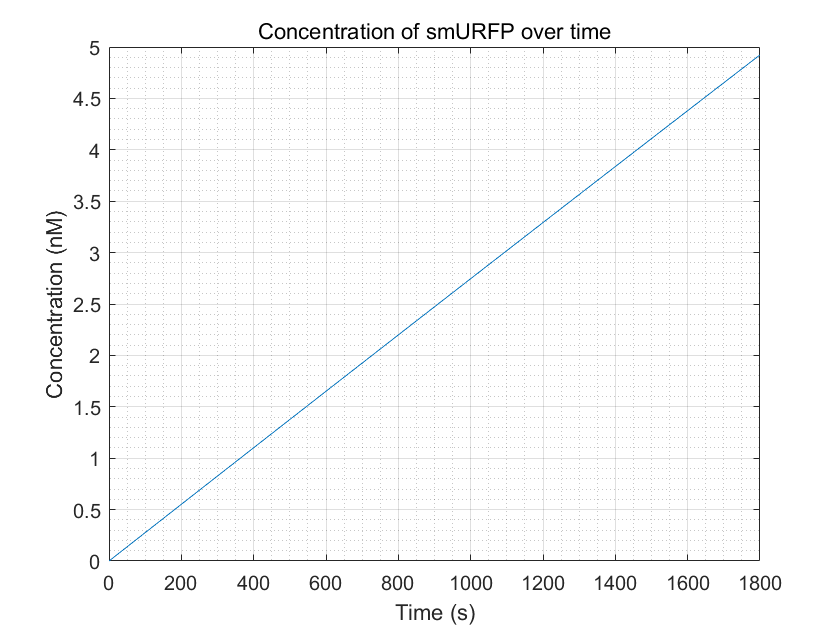
\includegraphics[width=7cm,height=7cm]{21}
	\caption{smURFP fluorescence reaches equilibrium but costs too long}
\end{figure}
From these three figures, we can conclude that dCas9-RNAP:sgRNA does have the effect of promoting transcription and increasing fluorescence intensity, thereby increasing sensitivity, as long as its concentration is sufficient. This result enhances the confidence of the experimental group, they just need to try to improve the expression of dCas9-RNAP:sgRNA in E. coli without having to doubt its role.



